\chapter{Experiments}\label{chapter:experiments}

In the present chapter, evaluation are performed on the approaches discussed in Chapter \ref{chapter:introduction} with the objective of identifying the most effective approach in the context of \gls{dva}. The appropriate selection of parameters is essential, as the primary objective in this context is to enhance signals originating from the vessel region. Moreover, the combination of different techniques can yield advantageous outcomes.

First, the discussion focuses on the results of \gls{clahe}, which is employed as a post-processing step for all the filtered images. Next, the outcomes of spatial domain filtering are examined. Then, the discussion focuses on the results of Fourier filtering. Additionally, the noise filtering characteristics of \gls{pca} are demonstrated in a subsection.

In order to test the efficiency of the techniques, the present thesis uses the following two DVA records:

\begin{figure}[htpb]
  \centering
  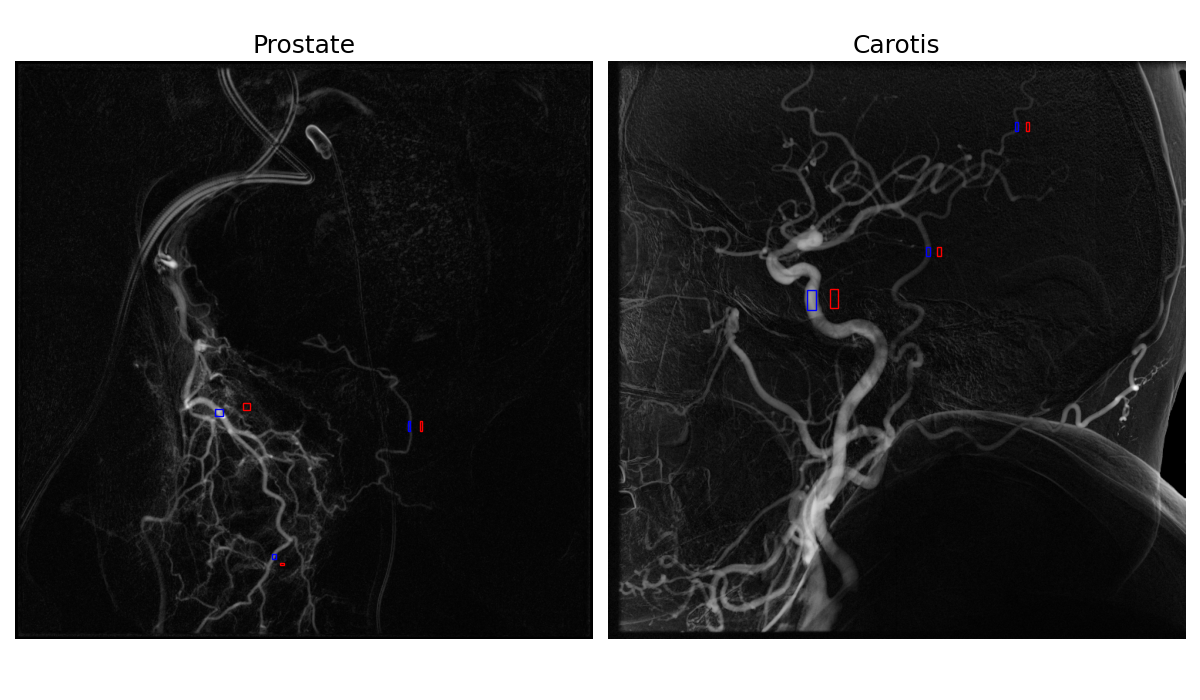
\includegraphics[width=0.9\textwidth]{figures/experiments/prostate-carotis-clahe.png}
  \caption{
	Sample \gls{dva} records with marked \gls{roi}s
   }
  \label{fig:prostate-carotis-clahe}
\end{figure}

The signal-to-noise ratio model used to perform quantitative analysis is as follows:
\begin{equation}
    SNR=\frac{\mu_{a} - \mu_{b}}{\sigma_{b}}
    \label{eq:snr}
\end{equation}

where $\mu_{a}$ is the signal mean measured in region of interest (\gls{roi}) $a$, $\mu_{b}$ is the signal mean measured in \gls{roi} $b$ and $\sigma_{b}$ is the standard deviation of the noise measure in \gls{roi} $b$. \gls{roi} $a$ areas are regions inside veins (colour blue on Figure \ref{fig:prostate-carotis}) while \gls{roi} $b$ areas are regions outside veins (colour red on Figure \ref{fig:prostate-carotis}). In an optimal scenario, a ROI $a$ is anticipated to yield a maximum signal, whereas a ROI $b$ is expected to yield no signal.

In addition to running SNR measurements, the evaluation of algorithm outcomes is performed by medical specialists too.

\section{Contrast Limited Adaptive Histogram Equalisation (\gls{clahe})}

As noted in Chapter \ref{subsection:intensity-transformations}, Contrast Limited Adaptive Histogram Equalisation (\gls{clahe}) is a highly effective technique due to its ability to do histogram equalisation on a local scale, namely on a tile-by-tile level. On Figure \ref{fig:prostate-carotis-clahe}, the \gls{clahe} enhanced image is displayed. In the absence of such enhancement, the \gls{dva} records would look as follows:

\begin{figure}[htpb]
  \centering
  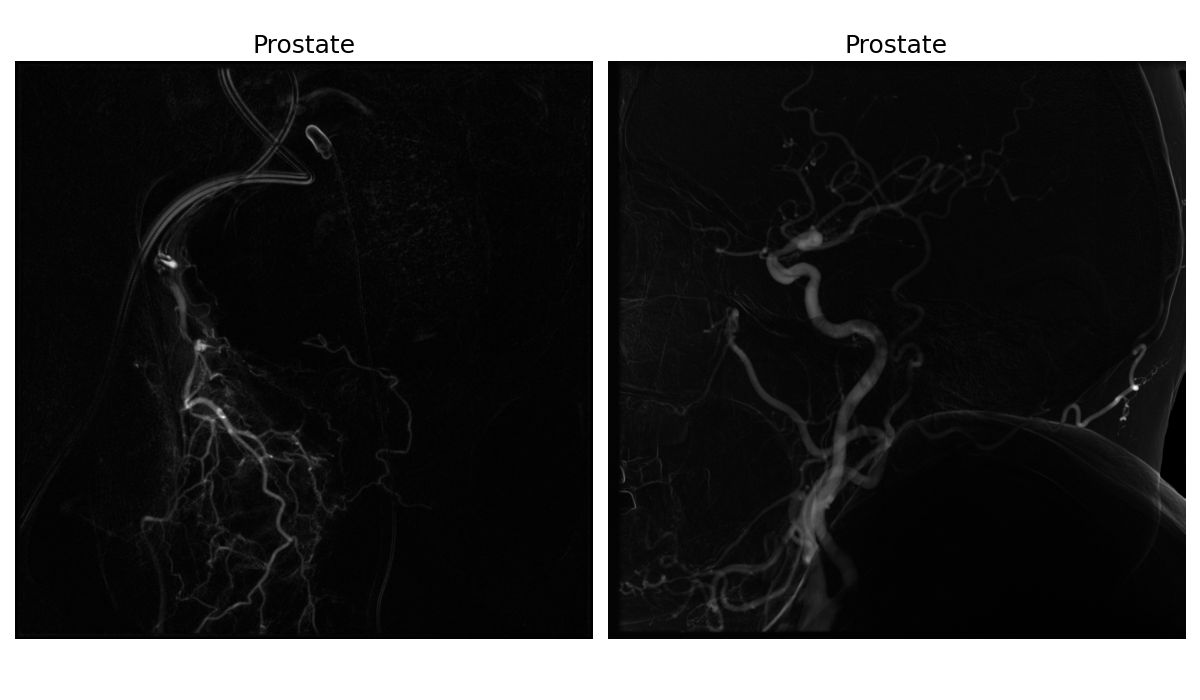
\includegraphics[width=0.9\textwidth]{figures/experiments/prostate-carotis.png}
  \caption{
	Records without \gls{clahe}
   }
  \label{fig:prostate-carotis}
\end{figure}

Following a series of intuitive experiments, the parameters were assigned the following values:
\begin{itemize}
	\item kernel\textunderscore size: set to the $1/10$ of image width and height
	\item clip\textunderscore limit: set to 0.00015 after rescaling the image to interval [0,1]	
\end{itemize}

All of the following images in the thesis were post-processed with the \gls{clahe}.

\section{Filtering in Spatial Domain}

\subsection{Sobel kernel}

As noted earlier, Sobel kernels are discretized gradient kernels with dimensions of 3x3. Typically, in the use of this method, a magnitude image is computed using Equation \ref{eq:sobel-magnitued}. 

\section{Principal Component Analysis (\gls{pca})}\label{section:pca}
